\subsection{Our proposed pointing strategies}
\label{sec:proposed_pointings}

For simplicity we chose to study one-year plans for an Extended
Mission, i.e., plans for Year 3 of the TESS mission. (Later in this
report we remark on some possible implications of our study for
additional years of an Extended Mission.)  Given the constraints
outlined in Sec.~\ref{sec:constraints_on_pointings}, we selected the
following options for detailed study:

\begin{figure*}[ht]
	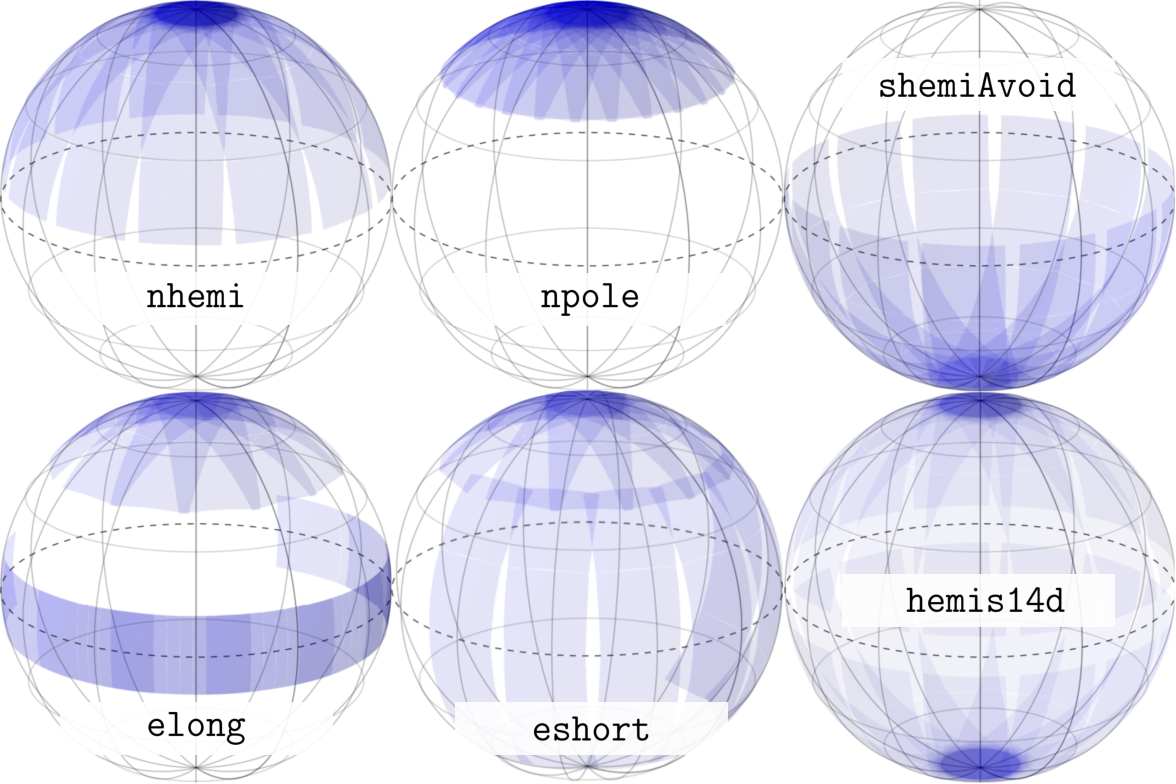
\includegraphics{figures/proposed_pointings_texttt.pdf}
	\caption{Proposed pointing strategies for a \tess Extended Mission, visualized in ecliptic coordinates. \nhemi, \npole, \shemiAvoid, \elong, \eshort, and \hemis. Note for \elong\:and \eshort\:that Earth and moon crossings likely make an entire year looking at the ecliptic impractical (see Fig.~\protect\ref{fig:earth_moon_elong}).}
	\label{fig:proposed_pointings}
\end{figure*}

\begin{description}

\item[Option 1.] \npole: Focus on one of the ecliptic poles,
  arbitrarily chosen to be the north ecliptic pole for
  concreteness. Note that the geometry of \tesss lens hood still
  suppresses incoming sunlight in this scenario.
  \textit{Justification:} maximizes the average duration of
  observations per star; intuitively we expected this to provide
  greatest sensitivity to long-period planets.

\item[Option 2.] \nhemi: Repeat observations of one of the two
  ecliptic hemispheres in a manner similar to the Primary Mission,
  arbitrarily chosen to be the northern ecliptic hemisphere for
  concreteness. In this scenario we could take the opportunity to 
  shift the longitudes of all sectors by an amount that would enable 
  TESS to cover the gaps that were left during the Primary Mission 
  (the ``slits'' in the sky coverage between ecliptic latitudes of 
  6--30$^\circ$).
  However for simplicity, we opted to observe the same longitudes as
  in the Primary Mission.
  \textit{Justification:} similar motivation as the Primary Mission.
  Nice long time baseline at the North Ecliptic Pole, and broad sky
  coverage. Also remeasures transit times (and sharpens ephemerides)
  of previously detected TESS planets over most of the entire
  hemisphere.

\item[Option 3.] \shemiAvoid: Repeat observations of one of the two
  ecliptic hemispheres, but in this case shifting all fields $6^\circ$
  toward the ecliptic, such that the combined fields-of-view reach all
  the way from the ecliptic to the ecliptic pole.
  \textit{Justification:} trades the long continuous viewing zone near
  the pole for greater sky coverage, and in particular, coverage of
  the ecliptic zone which was missed in the Primary Mission.  We chose
  to simulate the southern ecliptic hemisphere, since the northern
  version of this plan would suffer more from Earth-Moon interference
  (cf. Table~\ref{tab:dropped_fields} in
  Sec.~\ref{sec:earth_moon_crossings}).
  
\item[Option 4.] \elong: Survey the ecliptic with 7 sectors (14
  orbits) in which the long axis of the fields-of-view are oriented
  along the ecliptic.  For the other 6 sectors, during the interval
  when ecliptic observations would be interrupted by Earth-Moon
  crossings, we focus on one of the ecliptic poles.
  \textit{Justification:} covers the ecliptic, which was not surveyed
  at all in the Primary Mission.  Offers opportunities for follow-up
  of K2 discoveries. Minimizes Earth-moon interference.
  
\item[Option 5.] \eshort: Survey the ecliptic and also cover a large
  fraction of the rest of the ecliptic hemisphere. For 7 sectors we
  observe the ecliptic but with the {\it short} axis oriented along
  the ecliptic, and the long axis reaching up to higher latitudes.
  The remaining 6 sectors are focused on the ecliptic pole, as in
  \elong.  \textit{Justification:} similar to \elong, but with more
  overlap between this year and the Primary Mission to allow for
  improved transit ephemerides and better ability to follow-up on
  previous discoveries.
  
\item[Option 6.] \hemis: Cover both northern and southern ecliptic
  hemispheres in a single year, by alternating between the hemispheres
  every 13.7 days.  \textit{Justification:} rapid coverage of the
  entire sky, allows follow-up of almost all previously detected TESS
  objects and refined ephemerides.

\end{description}

Although these 6 seemed like good options for further study and direct
comparison, there are many other possibilities that may be of interest
that were not studied in detail, in order to keep the scope of this
report manageable.  Among these other possibilities that were considered but not studied are
\begin{itemize}
	\item The \npole\:strategy applied to the south ecliptic pole rather than the north (we do not expect major differences).
	\item The \nhemi\:strategy applied to the southern ecliptic hemipshere rather than the northern (we do not expect major differences).
	Similarly, the \nhemi\:strategy, but rotated about the ecliptic polar axis by
	$12^\circ$ in ecliptic longitude.
	\item The north/south inversion of \shemiAvoid, which is more strongly affected by Earth/Moon crossings (see Sec.~\ref{sec:earth_moon_crossings}).
	\item A full year spent observing the ecliptic.  It became clear that such a plan would suffer from Earth/Moon crossings for a substantial fraction of the year.
	We show the outage as a function of time in Fig.~\ref{fig:earth_moon_elong}.
        \item Alternate between northern and southern ecliptic poles every 13.7 days.
        This would be similar to \hemis\:but would focus on the poles rather than the entire sky.
        It would sacrifice sky coverage (and ability to refresh ephemerides over the whole sky) in return for longer-duration observations for a typical star.
        \item Hybrid strategies that change from month to month.  For instance, in the \nhemi\:scenario, during a month when the Earth or Moon crosses through the field of a camera pointed close to the ecliptic, we could tilt all the cameras away from the ecliptic as in the \npole\:scenario.        
\end{itemize}
